\documentclass[a4paper]{article}
\usepackage[T1]{fontenc}
\usepackage[english]{babel}
\usepackage{clrscode4e} % Algorithm template from Introduction to Algorithms 4th
\usepackage[left=2cm,right=2cm,top=1cm,bottom=2cm]{geometry} % page settings
\usepackage{amsthm, amsmath} % provides many mathematical environments & tools
\usepackage{tikz} % draw pictures
\usepackage{tabularray}
\usepackage[noend]{algorithmic}
\usepackage{tabularx}
\usepackage[noend]{algorithmic}
\usepackage{algorithm}
\usepackage{arydshln}
\usepackage{forest}
\usepackage{adjustbox}
\usepackage{array}
\usepackage{ifthen}
\usepackage{caption}
\usepackage{subfig}
\usepackage{graphicx,wrapfig,lipsum}
%-----------------------------------------------------------
% Custom commands
%-----------------------------------------------------------
\newenvironment{hashtable}[1][]
  {\begin{tabular}[#1]{
     @{}
     > {\small} r <{\normalsize~\rlap{\fbox{\strut~~}}$~~\rightarrow$~}
     @{} l @{}}}
  {\end{tabular}}

\tikzset{
node of list/.style = {
             draw,
             fill=orange!20,
             minimum height=6mm,
             minimum width=6mm,
             node distance=6mm
   },
link/.style = {
     -stealth,
     shorten >=1pt
     },
array element/.style = {
    draw, fill=white,
    minimum width = 6mm,
    minimum height = 10mm
  }
}

\def\LinkedList#1{%
  \foreach \element in \list {
     \node[node of list, right = of aux, name=ele] {\element};
     \draw[link] (aux) -- (ele);
     \coordinate (aux) at (ele.east);
  }
}

\usetikzlibrary{positioning,matrix, arrows.meta}
\tikzset{box/.style={draw, thick, minimum width=1cm, minimum height=1cm}}

\newenvironment{solution}
  {\begin{proof}[Solution]}
  {\end{proof}}
\renewcommand{\qedsymbol}{\rule{0.7em}{0.7em}}

\makeatletter
\renewenvironment{proof}[1][\proofname]{%
  \par\pushQED{\qed}\normalfont%
  \topsep6\p@\@plus6\p@\relax
  \trivlist\item[\hskip\labelsep\bfseries#1\@addpunct{.}]%
  \ignorespaces
}{%
  \popQED\endtrivlist\@endpefalse
}
\makeatother
\setlength{\parindent}{0mm}

%-----------------------------------------------------------
% Document
%-----------------------------------------------------------
\begin{document}

\title{Algorithms: Homework 2}
\author{Li-Yuan Wei}
\date{\today}
\maketitle

\subsection*{Problem 1}
\begin{solution}
$$
\begin{array}{cccc}
0(initial)& digit\ 1 & digit\ 2 & digit\ 3 \\\\
\hline
\text{NOD} & \text{EB$\textbf{B}$} & \text{B$\textbf{A}$N} & \text{$\textbf{A}$SH} \\\\
\text{HOG} & \text{NO$\textbf{D}$} & \text{B$\textbf{A}$R} & \text{$\textbf{B}$AN} \\\\
\text{SHY} & \text{TE$\textbf{D}$} & \text{P$\textbf{A}$R} & \text{$\textbf{B}$AR} \\\\
\text{BAN} & \text{HO$\textbf{G}$} & \text{E$\textbf{B}$B} & \text{$\textbf{E}$BB} \\\\
\text{BAR} & \text{FI$\textbf{G}$} & \text{T$\textbf{E}$D} & \text{$\textbf{F}$IG} \\\\
\text{JET} & \text{AS$\textbf{H}$} & \text{J$\textbf{E}$T} & \text{$\textbf{H}$OG} \\\\
\text{EBB} & \text{BA$\textbf{N}$} & \text{P$\textbf{E}$T} & \text{$\textbf{J}$ET} \\\\
\text{PAR} & \text{BA$\textbf{R}$} & \text{S$\textbf{H}$Y} & \text{$\textbf{N}$OD} \\\\
\text{ASH} & \text{PA$\textbf{R}$} & \text{F$\textbf{I}$G} & \text{$\textbf{P}$AR} \\\\
\text{PET} & \text{JE$\textbf{T}$} & \text{N$\textbf{O}$D} & \text{$\textbf{P}$ET} \\\\
\text{TED} & \text{PE$\textbf{T}$} & \text{H$\textbf{O}$G} & \text{$\textbf{R}$OT} \\\\
\text{ROT} & \text{RO$\textbf{T}$} & \text{R$\textbf{O}$T} & \text{$\textbf{S}$HY} \\\\
\text{FIG} & \text{SH$\textbf{Y}$} & \text{A$\textbf{S}$H} & \text{$\textbf{T}$ED} \\\\
\end{array}
$$
\end{solution}

\subsection*{Problem 2}
\begin{solution}
\end{solution}

\subsection*{Problem 3}
\begin{figure}[H]
\centering
\begin{minipage}{5cm}
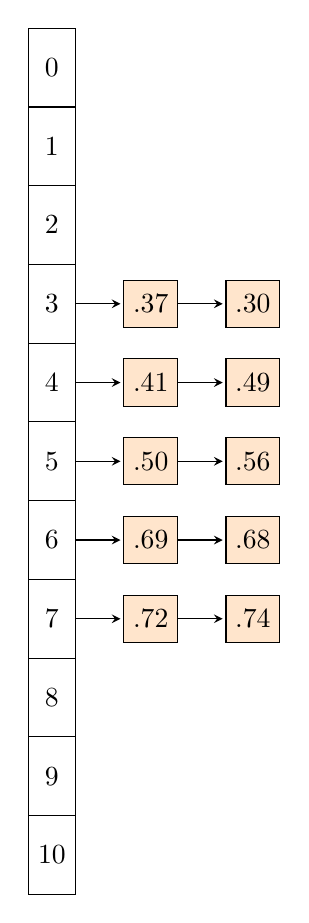
\begin{tikzpicture}
  \foreach \index/\list in {0/{}, 1/{}, 2/{}, 3/{.37,.30}, 4/{.41, .49}, 5/{.50, .56}, 6/{.69, .68}, 7/{.72, .74}, 8/{}, 9/{}, 10/{}} {
   \node[array element] (aux) at (0,-\index) {\index};
   \LinkedList{\list}
}
\end{tikzpicture}
\caption{Insert data}
\end{minipage}
\qquad
\begin{minipage}{5cm}
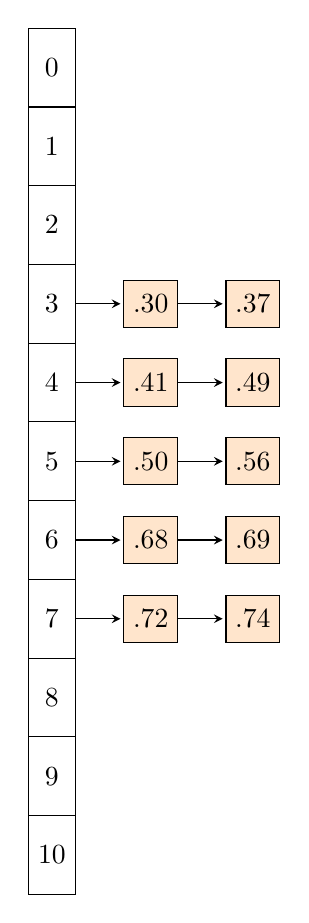
\begin{tikzpicture}
  \foreach \index/\list in {0/{}, 1/{}, 2/{}, 3/{.30,.37}, 4/{.41, .49}, 5/{.50, .56}, 6/{.68, .69}, 7/{.72, .74}, 8/{}, 9/{}, 10/{}} {
   \node[array element] (aux) at (0,-\index) {\index};
   \LinkedList{\list}
}
\end{tikzpicture}
\caption{Sort each bucket}
\label{bucket}
\end{minipage}
\end{figure}

\begin{solution}
To get sorted data, chain all in Figure \ref{bucket} from bucket $0$ to bucket $10$: \\
$<.30, .37, .41, .49, .50, .56, .68, .69, .72, .74>$
\end{solution}

\subsection*{Problem 4}
\begin{solution}
Psuedocode for finding the $k$-th smallest element:\\
\noindent
\begin{tabularx}{\textwidth}{>{\footnotesize}rX@{}}
  \\[-1.5ex] \hline
  \multicolumn{2}{@{}l}{\refstepcounter{algorithm}\label{find-k} $\proc{FIND-K-TH-SMALLEST}(X, k)$} \\
  \hline
   1: & \If $i > \attrib{A}{heap-size}$\\
   2: & \quad \Error $A[i]$ does not exist \\
   3: & key = $A[i]$ \\
   4: & $A[i] = A[\attrib{A}{heap-size}]$ \\
   5: & $\attrib{A}{heap-size} = \attrib{A}{heap-size} - 1$ \\
   6: & \If $A[i] <$ key \\
   7: & \quad $\proc{MAX-HEAPIFY}(A, i)$ \\
   8: & \textbf{else} \\
   9: & \quad key1 $= A[i]$ \\
  10: & \quad $A[i] =$ key \\
  11: & \quad $\proc{HEAP-INCREASE-KEY}(A, i, key1)$ \\
\hline
\\ [-0.2cm]
\end{tabularx}
\end{solution}

\subsection*{Problem 5}
\begin{solution}
Psuedocode for finding the median of arrays X and Y:\\
\noindent
\begin{tabularx}{\textwidth}{>{\footnotesize}rX@{}}
  \\[-1.5ex] \hline
  \multicolumn{2}{@{}l}{\refstepcounter{algorithm}\label{find-median} $\proc{FIND-MEDIAN}(X,Y,s,n)$} \\
  \hline
   1: & \If $i > \attrib{A}{heap-size}$\\
   2: & \quad \Error $A[i]$ does not exist \\
   3: & key = $A[i]$ \\
   4: & $A[i] = A[\attrib{A}{heap-size}]$ \\
   5: & $\attrib{A}{heap-size} = \attrib{A}{heap-size} - 1$ \\
   6: & \If $A[i] <$ key \\
   7: & \quad $\proc{MAX-HEAPIFY}(A, i)$ \\
   8: & \textbf{else} \\
   9: & \quad key1 $= A[i]$ \\
  10: & \quad $A[i] =$ key \\
  11: & \quad $\proc{HEAP-INCREASE-KEY}(A, i, key1)$ \\
\hline
\\ [-0.2cm]
\end{tabularx}
\end{solution}

\subsection*{Problem 6}
\begin{figure}[H]
\centering
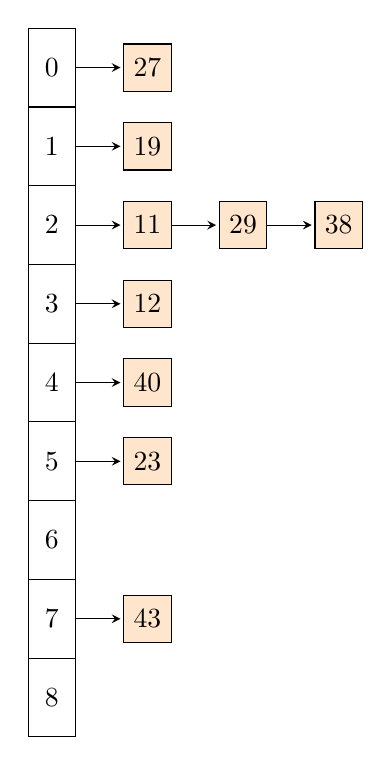
\begin{tikzpicture}
  \foreach \index/\list in {0/{27}, 1/{19}, 2/{11,29,38}, 3/{12}, 4/{40}, 5/{23}, 6/{}, 7/{43}, 8/{}} {
   \node[array element] (aux) at (0,-\index) {\index};
   \LinkedList{\list}
}
\end{tikzpicture}
\caption{Hash table with chaining}
\end{figure}

\subsection*{Problem 7}
\begin{figure}[H]
\centering
% 7.1 linear probing
\begin{minipage}{5cm}
\centering
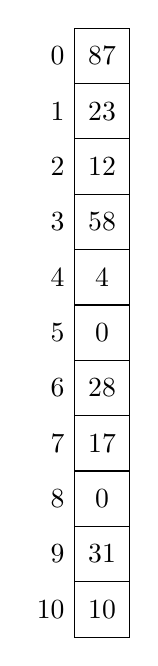
\begin{tikzpicture}
\coordinate (0);
\foreach \t[count=\i from 0,evaluate=\i as\j using int(\i+1)] in {
  87,
  23,
  12,
  58,
  4,
  0,
  28,
  17,
  0,
  31,
  10
}
\node at(\i.south)[anchor=north,draw,minimum height=2em,minimum width=2em,outer sep=0pt](\j){\t}
    node at(\j.west)[align=right,left]{\i}
    node at(\j.east)[align=left,right,xshift=-.7em]{};
\end{tikzpicture}
\caption{linear probing}
\end{minipage}
\qquad
% 7.2 quadratic hashing
\begin{minipage}{5cm}
\centering
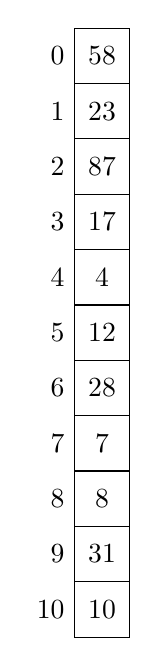
\begin{tikzpicture}
\coordinate (0);
\foreach \t[count=\i from 0,evaluate=\i as\j using int(\i+1)] in {
  58,
  23,
  87,
  17,
  4,
  12,
  28,
  7,
  8,
  31,
  10
}
\node at(\i.south)[anchor=north,draw,minimum height=2em,minimum width=2em,outer sep=0pt](\j){\t}
    node at(\j.west)[align=right,left]{\i}
    node at(\j.east)[align=left,right,xshift=-.7em]{};
\end{tikzpicture}
\caption{quadratic probing}
\end{minipage}
\qquad
% 7.3 double hashing
\begin{minipage}{5cm}
\centering
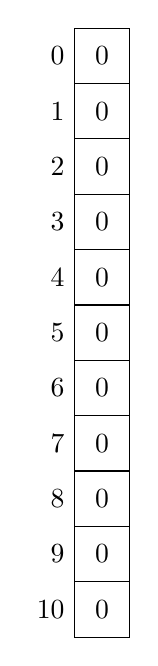
\begin{tikzpicture}
\coordinate (0);
\foreach \t[count=\i from 0,evaluate=\i as\j using int(\i+1)] in {
  0,
  0,
  0,
  0,
  0,
  0,
  0,
  0,
  0,
  0,
  0
}
\node at(\i.south)[anchor=north,draw,minimum height=2em,minimum width=2em,outer sep=0pt](\j){\t}
    node at(\j.west)[align=right,left]{\i}
    node at(\j.east)[align=left,right,xshift=-.7em]{};
\end{tikzpicture}
\caption{double hashing}
\end{minipage}
\end{figure}

\subsection*{Problem 8}
\begin{solution}
\end{solution}

\subsection*{Problem 9}
\begin{solution}
\end{solution}

\subsection*{Problem 10}
\begin{solution}
\end{solution}

\end{document}


